\documentclass[12pt,letterpaper]{article}
\usepackage{graphicx,textcomp}
\usepackage{natbib}
\usepackage{setspace}
\usepackage{fullpage}
\usepackage{color}
\usepackage[reqno]{amsmath}
\usepackage{amsthm}
\usepackage{fancyvrb}
\usepackage{amssymb,enumerate}
\usepackage[all]{xy}
\usepackage{endnotes}
\usepackage{lscape}
\newtheorem{com}{Comment}
\usepackage{float}
\usepackage{hyperref}
\newtheorem{lem} {Lemma}
\newtheorem{prop}{Proposition}
\newtheorem{thm}{Theorem}
\newtheorem{defn}{Definition}
\newtheorem{cor}{Corollary}
\newtheorem{obs}{Observation}
\usepackage[compact]{titlesec}
\usepackage{dcolumn}
\usepackage{tikz}
\usetikzlibrary{arrows}
\usepackage{multirow}
\usepackage{xcolor}
\newcolumntype{.}{D{.}{.}{-1}}
\newcolumntype{d}[1]{D{.}{.}{#1}}
\definecolor{light-gray}{gray}{0.65}
\usepackage{url}
\usepackage{listings}
\usepackage{color}

\definecolor{codegreen}{rgb}{0,0.6,0}
\definecolor{codegray}{rgb}{0.5,0.5,0.5}
\definecolor{codepurple}{rgb}{0.58,0,0.82}
\definecolor{backcolour}{rgb}{0.95,0.95,0.92}

\lstdefinestyle{mystyle}{
	backgroundcolor=\color{backcolour},   
	commentstyle=\color{codegreen},
	keywordstyle=\color{magenta},
	numberstyle=\tiny\color{codegray},
	stringstyle=\color{codepurple},
	basicstyle=\footnotesize,
	breakatwhitespace=false,         
	breaklines=true,                 
	captionpos=b,                    
	keepspaces=true,                 
	numbers=left,                    
	numbersep=5pt,                  
	showspaces=false,                
	showstringspaces=false,
	showtabs=false,                  
	tabsize=2
}
\lstset{style=mystyle}
\newcommand{\Sref}[1]{Section~\ref{#1}}
\newtheorem{hyp}{Hypothesis}

\title{Problem Set 2}
\date{
	Name: Darragh McGee (18319331)\\
}
\author{Applied Stats/Quant Methods 1}
	
	\vspace{.5cm}
	
\begin{document}
	\maketitle
	
\vspace{1cm}
	\section*{Question 1: Political Science}
		\vspace{0.5cm}
	The following table was created using the data from a study run in a major Latin American city.\footnote{Fried, Lagunes, and Venkataramani (2010). ``Corruption and Inequality at the Crossroad: A Multimethod Study of Bribery and Discrimination in Latin America. \textit{Latin American Research Review}. 45 (1): 76-97.} As part of the experimental treatment in the study, one employee of the research team was chosen to make illegal left turns across traffic to draw the attention of the police officers on shift. Two employee drivers were upper class, two were lower class drivers, and the identity of the driver was randomly assigned per encounter. The researchers were interested in whether officers were more or less likely to solicit a bribe from drivers depending on their class (officers use phrases like, ``We can solve this the easy way'' to draw a bribe). The table below shows the resulting data.
\vspace{1cm}
\begin{table}[h!]
	\centering
	\begin{tabular}{l | c c c }
		& Not Stopped & Bribe requested & Stopped/given warning \\
		\\[-1.8ex] 
		\hline \\[-1.8ex]
		Upper class & 14 & 6 & 7 \\
		Lower class & 7 & 7 & 1 \\
		\hline
	\end{tabular}
\end{table}

\newpage
\begin{enumerate}
	\item [(a)]
	Calculate the $\chi^2$ test statistic by hand/manually (even better if you can do "by hand" in \texttt{R}).\\
\end{enumerate}
\noindent\textbf{Step 1:} Assumptions
\begin{itemize}
	\item 
	The data consists of categorical variables (social class and type of police interaction)
	\item
	The data is from a random sample. 
	\item 
	Observations are independent (one observation does not influence another).
\end{itemize}

\noindent The two variables are independent if the conditional distributions across categories are identical.
\vspace{0.5cm}

\noindent\textbf{Step 2:} Setting Up Hypothesis
\begin{itemize}
	\item 
	\textbf{Null Hypothesis:} The relationship between social class and the type of police interaction is statistically independent.
	\item
	\textbf{Alternative Hypothesis:} The relationship between social class and the type of police interaction is statistically dependent.
\end{itemize}

\vspace{0.5cm}
\noindent\textbf{Step 3:} Calculate the Test Statistic

\begin{center}
	 $\chi^2 = \sum \frac{(O_i - E_i)^2}{E_i}$
\end{center}

\noindent Chi-Squared is equal to the sum of the squared difference between the observed frequency and expected frequency, divided by the expected frequency for each cell in the contingency table.

\vspace{.5cm}
\noindent Create the Observed Frequency Table in R 
\lstinputlisting[language=R, firstline=28, lastline=29]{PS02_answers_DMcG.R}
\lstinputlisting[language=R, firstline=31, lastline=33]{PS02_answers_DMcG.R}
\lstinputlisting[language=R, firstline=35, lastline=35]{PS02_answers_DMcG.R}

\vspace{0.5cm}
\noindent Formula to Calculate the Expected Frequency
\[
\text{Expected frequency}_{ij} = \frac{\text{Row total}_i \times \text{Column total}_j}{\text{Grand total}}
\]

\newpage
\vspace{0.5cm}
\noindent Calculate the Row Totals
\lstinputlisting[language=R, firstline=41, lastline=42]{PS02_answers_DMcG.R}

\begin{verbatim}
Upper class Lower class 
27          15
\end{verbatim}

\vspace{0.5cm}
\noindent Calculate the Column Totals
\lstinputlisting[language=R, firstline=45, lastline=46]{PS02_answers_DMcG.R}

\begin{verbatim}
Not Stopped    Bribe Requested	  Stopped/Given Warning 
21             13                 8 
\end{verbatim}

\vspace{0.5cm}
\noindent Calculate the Grand Total
\lstinputlisting[language=R, firstline=49, lastline=50]{PS02_answers_DMcG.R}

\begin{verbatim}
Grand Total = 42
\end{verbatim}

\vspace{0.5cm}
\noindent Calculate the Expected Frequency
\lstinputlisting[language=R, firstline=53, lastline=54]{PS02_answers_DMcG.R}

\begin{verbatim}
     Not Stopped   Bribe Requested    Stopped/Given Warning
[1,] 13.5          8.357143           5.142857
[2,] 7.5           4.642857           2.857143
\end{verbatim}

\vspace{0.5cm}
\noindent Calculate the Test Statistic using Chi-Squared Formula
\lstinputlisting[language=R, firstline=57, lastline=59]{PS02_answers_DMcG.R}

\begin{verbatim}
Chi-Squared Statistic = 3.791168
\end{verbatim}

\newpage
\begin{enumerate}
	\item [(b)]
	Now calculate the p-value from the test statistic you just created. What do you conclude if $\alpha = 0.1$?\\
\end{enumerate}

\noindent\textbf{Step 4:} Calculate the p-value

\vspace{0.5cm}
\noindent Calculate the Degrees of Freedom
\[
\text{Degrees of freedom} = (\text{Number of rows} - 1) \times (\text{Number of columns} - 1)
\]
\lstinputlisting[language=R, firstline=66, lastline=66]{PS02_answers_DMcG.R}

\vspace{0.5cm}
\noindent\ Chi-Squared p-value Formula in R
\lstinputlisting[language=R, firstline=68, lastline=69]{PS02_answers_DMcG.R}
\begin{verbatim}
p-value = 0.1502306
\end{verbatim}

\vspace{0.5cm}
\noindent\textbf{Step 5:} Conclusion
\begin{itemize}
	\item 
	The p-value (0.1502306) is greater than the significance level of 0.1. Therefore, there is insufficient evidence to reject the null hypothesis that social class and the type of police interaction are statistically independent.
	\item
	In other words, we cannot conclude that there is a statistically significant relationship between social class and police interactions based on this data.
\end{itemize}

\newpage
\vspace{1cm}
\begin{enumerate}
\item [(c)] Calculate the standardized residuals for each cell and put them in the table below.
\end{enumerate}
\vspace{0.5cm}	
\noindent\ Standardised Residual Formula:
\vspace{0.5cm}
\[
z = \frac{\text{Observed frequency} - \text{Expected frequency}}{\sqrt{\text{Expected frequency}}}
\]

\vspace{0.5cm}
\noindent\ Standardised Residual refers to how far away each observation is from expectation. 
\vspace{0.5cm}

\noindent\ Standardised Residual Calculation:
\vspace{0.5cm}
\lstinputlisting[language=R, firstline=84, lastline=86]{PS02_answers_DMcG.R}

\vspace{0.5cm}
\noindent\ Table of Standardised Residual Output Summary:
	\begin{table}[h]
		\centering
		\begin{tabular}{l | c c c }
			& Not Stopped & Bribe requested & Stopped/given warning \\
			\\[-1.8ex] 
			\hline \\[-1.8ex]
			Upper class  & 0.1360828  & -0.8153742 & 0.818923 \\
			\\
			Lower class & -0.1825742 & 1.0939393  &  -1.098701 \\
			
		\end{tabular}
	\end{table}
	
\newpage
\begin{enumerate}
	\item [(d)] How might the standardized residuals help you interpret the results?  	
\end{enumerate}

\begin{itemize}
	\item 
	 The expected frequency represents the values that would be expected in each cell of a contingency table if the two categorical variables were independent.
	\item
	Standardised residuals measure how much the observed frequencies deviate from the expected frequencies, helping to identify which cells contribute most to the Chi-squared statistic. 
	\item 
	Larger standardised residuals indicate greater deviations from expected frequencies, while smaller residuals suggest the observed and expected values are similar.
	\item 
	In this analysis, the residuals for "Not Stopped" (e.g., 0.136 and -0.183) are small, indicating minimal deviations from expected values and contributing little to the Chi-squared statistic. 
	\item 
	For "Bribe Requested" (e.g., -0.815 and 1.094) and "Stopped or Given Warning" (e.g., 0.819 and -1.099), the residuals suggest moderate deviations from expected values.
	\item 
	None of the standardised residuals provide substantial evidence of deviations from independence. As a result, these residuals support a higher p-value and reinforce the conclusion that there is insufficient evidence to reject the null hypothesis.
\end{itemize}

\newpage
\section*{Question 2: Economics}
Chattopadhyay and Duflo were interested in whether women promote different policies than men.\footnote{Chattopadhyay and Duflo. (2004). ``Women as Policy Makers: Evidence from a Randomized Policy Experiment in India. \textit{Econometrica}. 72 (5), 1409-1443.} Answering this question with observational data is pretty difficult due to potential confounding problems (e.g. the districts that choose female politicians are likely to systematically differ in other aspects too). Hence, they exploit a randomized policy experiment in India, where since the mid-1990s, $\frac{1}{3}$ of village council heads have been randomly reserved for women. A subset of the data from West Bengal can be found at the following link: \url{https://raw.githubusercontent.com/kosukeimai/qss/master/PREDICTION/women.csv}\\

\noindent Each observation in the data set represents a village and there are two villages associated with one GP (i.e. a level of government is called "GP"). Figure~\ref{fig:women_desc} below shows the names and descriptions of the variables in the dataset. The authors hypothesize that female politicians are more likely to support policies female voters want. Researchers found that more women complain about the quality of drinking water than men. You need to estimate the effect of the reservation policy on the number of new or repaired drinking water facilities in the villages.
\vspace{.5cm}
\begin{figure}[h!]
	\caption{\footnotesize{Names and description of variables from Chattopadhyay and Duflo (2004).}}
	\vspace{.5cm}
	\centering
	\label{fig:women_desc}
	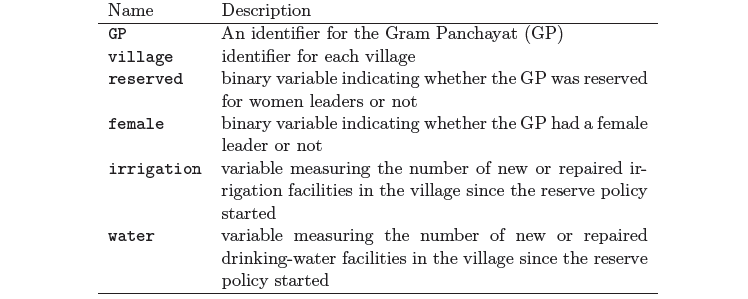
\includegraphics[width=1.1\textwidth]{women_desc.png}
\end{figure}		

\newpage
\begin{enumerate}
	\item [(a)] State a null and alternative (two-tailed) hypothesis. 
\end{enumerate}
\noindent\textbf{Step 1:} Assumptions about the Data
\begin{itemize}
	\item 
	Linear relationship: There is a linear relationship between the explanatory  and response variables.
	\item
	Independence: The observations are independent of each other.
	\item 
	Normally Distributed Errors: For any given value of the explanatory variable, the errors (residuals) are assumed to follow a normal distribution.
	\item 
	Constant variance (Homoscedasticity): The variance of the errors is constant across all values of the independent variable.
\end{itemize}

\noindent\textbf{Step 2:} Setting Up Hypothesis
\begin{itemize}
	\item 
	\textbf{Null Hypothesis:} The policy of reserving village council head positions for women does not affect the number of new or repaired drinking-water facilities in the village. ($\beta = 0$)
	\item
	\textbf{Alternative Hypothesis:} The policy of reserving village council head positions for women does affect the number of new or repaired drinking-water facilities in the village. ($\beta \neq 0$)
\end{itemize}

\newpage
\begin{enumerate}
	\item [(b)] Run a bivariate regression to test this hypothesis in \texttt{R} (include your code!).
\end{enumerate}
\vspace{.5cm}
\noindent Load Relevant Data: 
\lstinputlisting[language=R, firstline=130, lastline=131]{PS02_answers_DMcG.R}
\vspace{.5cm}
\noindent Operationalise the Relevant Variables:
\lstinputlisting[language=R, firstline=133, lastline=134]{PS02_answers_DMcG.R}
\vspace{.5cm}
\noindent Create a Scatterplot to Visualise the Relationship: 
\lstinputlisting[language=R, firstline=136, lastline=143]{PS02_answers_DMcG.R}

\begin{figure}[H]
	\centering
	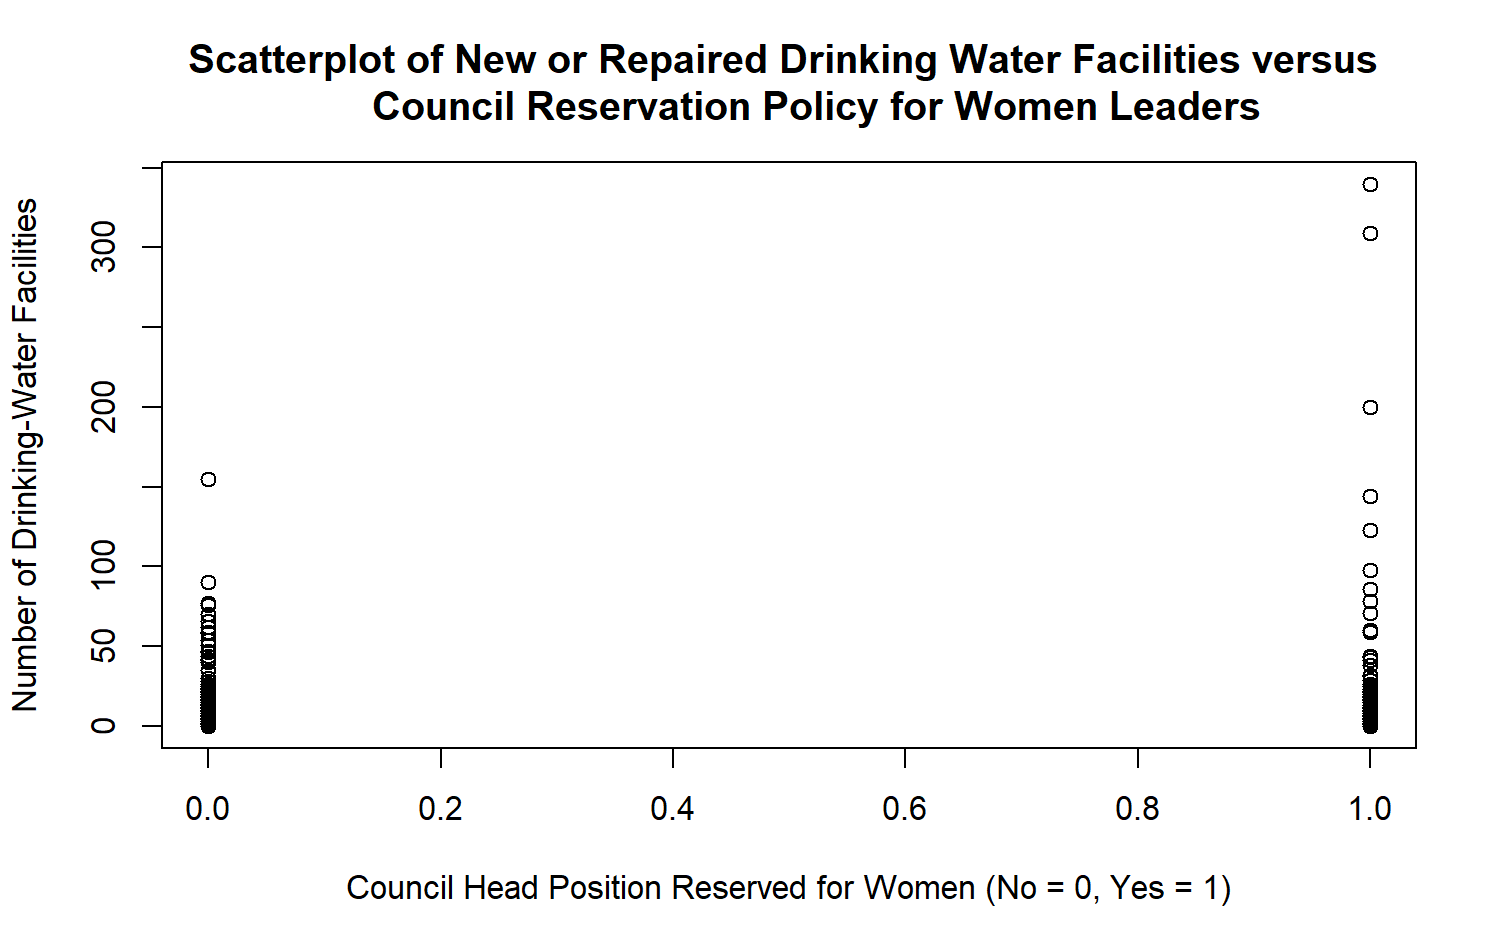
\includegraphics[width=0.8\textwidth]{Figure_2_1.png}
\end{figure}

\noindent Run Bivariate Regression Analysis 
\lstinputlisting[language=R, firstline=145, lastline=147]{PS02_answers_DMcG.R}

\noindent Bivariate Regression Analysis Output:
\begin{verbatim}
Residuals:
Min        1Q        Median   3Q       Max 
-23.991    -14.738   -7.865   2.262    316.009 

Coefficients:
              Estimate Std.  Error    t value    Pr(>|t|)    
(Intercept)   14.738         2.286    6.446      4.22e-10 ***
X              9.252         3.948    2.344      0.0197 *  
---
Signif. codes:  0 ‘***’ 0.001 ‘**’ 0.01 ‘*’ 0.05 ‘.’ 0.1 ‘ ’ 1
\end{verbatim}
\vspace{.5cm}
\noindent\textbf{Step 3:} Calculate Test Statistic

\noindent t-statistic available from R Summary Model

\begin{verbatim}
	t-value = 2.344
\end{verbatim}
\vspace{.5cm}
\noindent\textbf{Step 4:} Calculate p-value

\noindent p-value available from R Summary Model

\begin{verbatim}
	p-value = 0.0197
\end{verbatim}
\vspace{.5cm}
\noindent\textbf{Step 5:} Conclusion 
\begin{itemize}
	\item 
	In a bivariate regression analysis, the slope represents both the strength and direction of the relationship between two variables (an explanatory and response variable). Specifically, in this analysis, the slope illustrates how the policy of reserving village council head positions for women impacts the number of new or repaired drinking-water facilities in the village.
	\item
	If the slope is statistically significantly different from 0, it indicates a relationship between the two variables. In this case, the p-value is 0.0197, which is statistically significant at the 95 percent confidence level ($\alpha < 0.05$).
	\item 
	Therefore, we reject the null hypothesis that the policy of reserving village council head positions for women has no effect on the number of new or repaired drinking-water facilities.
	\item 
	There is sufficient evidence to conclude that the reservation policy has an impact on the number of new or repaired drinking-water facilities in the village.
\end{itemize}

\newpage
\begin{enumerate}
	\item [(c)] Interpret the coefficient estimate for reservation policy. 
\end{enumerate}
\vspace{0.5cm}
\begin{itemize}
	\item 
	The coefficient for the reservation policy is 9.252, which represents the slope of the relationship between the reservation policy and the number of new or repaired drinking-water facilities in the village. This coefficient explains how a one-unit change in the explanatory variable (reservation policy) affects the response variable (number of drinking-water facilities).
	\item
	The coefficient is positive meaning that the reservation policy is associated with an increase in the number of new or repaired drinking-water facilities.
	\item
	The reservation policy is a binary variable (coded as 0 for no reservation policy and 1 for reservation policy). This indicates that, villages that have implemented the reservation policy tend to have approximately 9.252 more new or repaired drinking-water facilities on average when compared to villages that have no reservation policy. 
\end{itemize}
\end{document}
